\documentclass[12pt,pra,aps]{revtex4}
\usepackage[dvipdfmx]{graphicx}
\usepackage[dvipdfmx]{color}
\usepackage[version=3]{mhchem}
\usepackage{float}
\usepackage{rotating}
\usepackage{array}
\usepackage{amsmath}
\usepackage{multirow}
\usepackage{setspace}
\usepackage{braket}
\usepackage{epstopdf}
\usepackage{moreverb}
\usepackage{wrapfig}

\usepackage{color}                            
                                              
\newcommand{\red}[1]{\textcolor{red}{#1}}     
\newcommand{\blue}[1]{\textcolor{blue}{#1}}

\newcommand{\boxz}[1]{\boxed{\phantom{\text{#1}}}}
\newcommand{\boxa}[1]{\boxed{\phantom{}}}

%%\renewcommand{\baselinestretch}{2.0}

\renewcommand{\thefigure}{S\arabic{figure}}
\renewcommand{\thetable}{S\arabic{table}}

\begin{document}
\title{分子軌道と分子の構造 \\(水素分子イオンとH\"uckel分子軌道法)}
\author{齋藤 雅明 \\ 量子化学研究室 \\ email: masa.saitow@chem.nagoya-u.ac.jp}

\maketitle

\noindent
{\bf 問題1.} 以下の文を読んで、空欄を埋めよ。

\noindent
水素分子イオンの基底量子状態を考える。水素分子イオンは、正電荷を持つ二つの\boxz{陽子}と一つの電子からなる。Hamiltonian演算子の\boxz{最低固有}を持つ固有関数として与えられる基底状態波動関数は、電子と原子核両方の座標に依存する関数であるが、\boxz{Born-Oppenheimer}近似を用いることで、原子核部分と電子部分とに分離される。この近似に基づく、非相対論的電子Hamiltonian演算子は原子単位で\boxz{$H=-\frac{1}{2}\nabla^2-\frac{1}{r_\text{A}}-\frac{1}{r_\text{B}}+\frac{1}{R}$}と与えられる。水素分子イオンの量子状態は、厳密には\boxz{3}体問題であり、厳密解は得られない。しかしながらこの近似により、時間\text{非依存}シュレーディンガー方程式は、実効的な\boxz{1}体問題へと帰着され、解析的な求解が可能となる。この近似に基づく水素分子イオンの電子波動関数は数学的には非常に複雑となり、直感的に電子状態を理解するのは困難である。そこで、二つの水素原子軌道関数の重ね合わせとして表現し、重ね合わせの係数を\boxz{変分}原理に基づき最適化する。これを\boxz{LCAO}-MO法という。

% Nakai & Ando, p. 68
\noindent
{\bf 問題2.} 1,3-ブタジエンとシクロブタジエンの共鳴安定化をH\"uckel法により考察する。
    
\noindent
{\bf 2.(a)} ブタジエンに対する永年方程式を解き、4つのエネルギー準位を求めよ。また、それぞれのエネルギー準位に対する占有状態も答えよ。

\noindent
{\bf 2.(b)} ブタジエンの$\pi$電子の全エネルギー及び共鳴エネルギー\footnote{非局在化エネルギーとも呼ばれる。}を求めよ。

\noindent
{\bf 2.(c)} シクロブタジエンに対する永年方程式を解き、4つのエネルギー準位を求めよ。また、それぞれのエネルギー準位に対する占有状態も答えよ。

\noindent
{\bf 2.(d)} シクロブタジエンの$\pi$電子の全エネルギー及び共鳴エネルギーを求めよ。

\noindent
{\bf 2.(e)} ブタジエン及シクロブタジエンの全結合次数を計算せよ。

% Nakai & Ando, p. 69
\noindent
{\bf 問題3.} ベンゼン\ce{C6H6}の$\pi$電子状態をH\"uckel法により考察する。

\noindent
{\bf 3.(a)} ベンゼンに対する永年方程式を解き、4つのエネルギー準位を求めよ。また、それぞれのエネルギー準位に対する占有状態も答えよ。

\noindent
{\bf 3.(b)} ベンゼンの6個の$\pi$電子は(a)で求めたエネルギー準位をどのように占有するか模式的に示せ。

\noindent
{\bf 3.(c)} ベンゼンの全エネルギー及び共鳴エネルギーを求めよ。

\begin{wrapfigure}{r}[9pt]{0.2\textwidth}
  \centering
  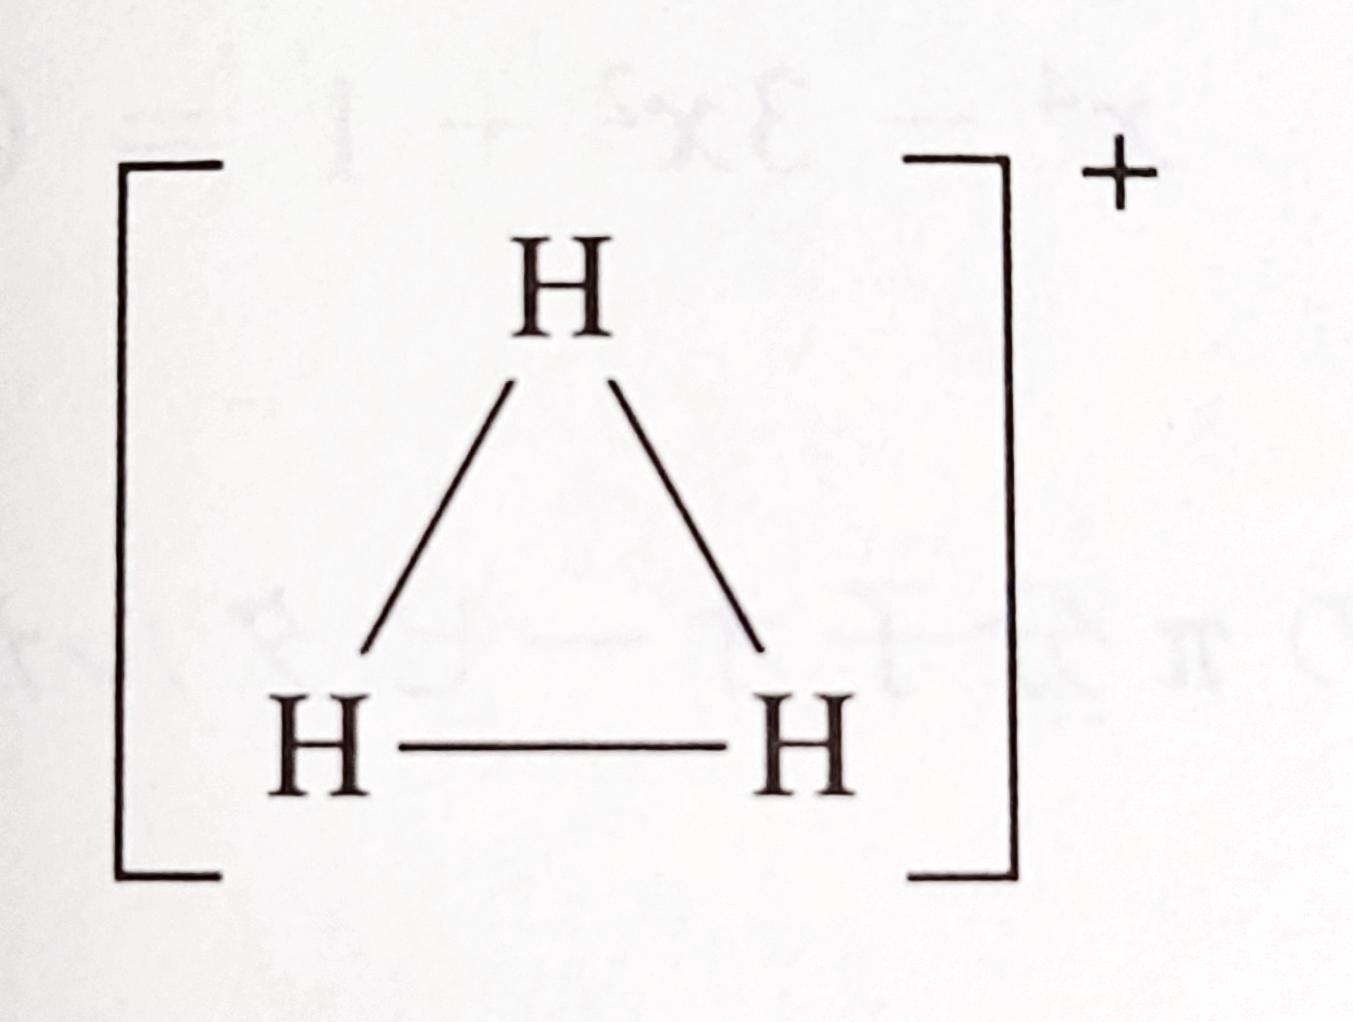
\includegraphics[width=3.0cm]{triangle.jpg}
  \caption{Triangular structure of \ce{H3+} molecule}
\end{wrapfigure}

\noindent
{\bf 3.(d)} ベンゼンのイオン化エネルギー及び電子親和力を求めよ。

\noindent
{\bf 3.(e)} ベンゼンの共鳴エネルギーの実測値は209 kJ/mol${}^{-1}$である。この数値を再現するように、共鳴積分の値を決定せよ。また1,3-ブタジエンの共鳴エネルギーの実測値は43 kJ/mol${}^{-1}$である。このように決定された共鳴積分を用いた場合、エチレンの共鳴エネルギーはどのようになるか。

% McQuarrie p. 440, Prob. 10.37
\noindent
{\bf 問題4.} H\"uckel法によって、\ce{H3+}について直線構造と三角形構造のどちらが安定かを決定せよ。\ce{H3}と\ce{H3-}ではどうか。

\end{document}
